\documentclass[12pt]{article}
\usepackage[spanish]{babel}
\usepackage[left=2.5cm,top=2.0cm,right=2.5cm,bottom=3.0cm]{geometry}
\usepackage[utf8]{inputenc}
\usepackage{url} % ACENTOS
\usepackage{graphicx}
\usepackage{fancyhdr}
\usepackage{xcolor}
\usepackage{multirow}
\usepackage{listings}
\usepackage{caption}
\usepackage{subcaption}
\usepackage{pdfpages} % Incluir PDF en documento en LATEX
\usepackage[backend=bibtex,sorting=none]{biblatex}
\setcounter{biburllcpenalty}{7000}
\setcounter{biburlucpenalty}{8000}
\addbibresource{referencias.bib} % ARCHIVO DE BIBLIOGRAFÍA
\usepackage[bookmarks=true,breaklinks=true,bookmarksopen=false,colorlinks=true,linkcolor=blue]{hyperref}
\usepackage[hyphenbreaks]{breakurl}
\usepackage{datetime}
\newdateformat{specialdate}{\twodigit{\THEDAY}-\twodigit{\THEMONTH}-\THEYEAR}
%\newdateformat{specialdate}{\twodigit{\THEDAY}-\THEYEAR}
\date{\specialdate\today}
\newcommand{\HRule}{\rule{\linewidth}{0.25mm}}
% CONSTANTES NECESARIAS PARA EL DOCUMENTO ---> MODIFIQUEN A SU CRITERIO
\newcommand{\elola}        {el}  %Hombres cambien LA por EL
\newcommand{\OA}           {o}  %Hombres cambien A por O
\newcommand{\ncuatrimestre}{Enero-Abril 2018}

\newcommand{\nproyecto}           {Sistema de envío de recomendaciones para la concientización de la diabetes en personas adultas.}

\newcommand{\nproyectoheader}     {Chatbot para la concientización de la Diabetes}
\newcommand{\nalumnoA}            {Wbario, Torres, Rojas, Echartea y Muñiz}
\newcommand{\ncarrera}            {Ingeniería en Tecnologías de la Información}
\newcommand{\nasesorinstitucional}{Dr. Hector Hugo Áviles Arriaga}
\newcommand{\fecha}               {Septiembre de 2018}
\newcommand{\fechacarta}		  {12 de Septiembre de 2017}
\newcommand{\separacionCorta}{0.0cm}
\newcommand{\separacionLarga}{0.5cm}
\usepackage[overload]{textcase}
\newcommand{\iemph}[1]{\MakeTextUppercase{#1}}
\pagestyle{fancy}
\headheight 35pt
\fancyhead{} % Clear all header fields
\fancyhead[L]{
\includegraphics[height=1.5cm]{figuras/CGUTP2.png}}%
\fancyhead[C]{\nproyectoheader}%
\fancyhead[R]{
\includegraphics[height=1.5cm]{figuras/LogoUPV.png}}%
\fancyfoot[R]{\thepage} % Clear all footer fields 
\fancyfoot[C]{}
\fancyfoot[L]{}
\DefineBibliographyStrings{english}{%
  references = {Referencias},% replace "references" with "bibliography"  for `book`/`report`
}
\addto\captionsenglish{%
  \renewcommand{\figurename}{Figura}%
  \renewcommand{\tablename}{Cuadro}%
} 
\usepackage{wallpaper}
\begin{document}
%-----------------------------------------------------------------------------------------------------------------
% PAGINA 1 - PORTADA
\setcounter{page}{1}
\pagenumbering{roman}
\thispagestyle{empty}
\begin{center}
\begin{tabular}{cp{8cm}c}

\includegraphics[height=2.25cm]{figuras/CGUTP2.png} & 
& 
\includegraphics[height=2.25cm]{figuras/LogoUPV.png}   \\
\end{tabular}
\Large \textbf{UNIVERSIDAD POLITÉCNICA DE VICTORIA}
\vspace{0.5cm}
\hrule
\vspace{0.1cm}
\hrule
\vspace{2.0cm}
\textbf{\iemph{\nproyecto}} \\[\separacionLarga]
CARRERA: \\
\textbf{\iemph{\ncarrera}} \\[\separacionLarga]
\vspace{1cm}
PRESENTAN: \\[\separacionCorta]
\textbf{\iemph{\nalumnoA}}\\[\separacionLarga]
\vspace{1.5cm}
REVISOR: \\[\separacionCorta]
\textbf{\iemph{\nasesorinstitucional}} \\[\separacionCorta]
\vspace{2.0cm}
\end{center}
\begin{flushright}
\iemph{Ciudad Victoria, Tamaulipas, \fecha}
\end{flushright}
\HRule 
%-----------------------------------------------------------------------------------------------------------------
% PAGINA 5 - RESUMEN EN ESPAÑOL
\clearpage
\section*{\centering Resumen}
\addcontentsline{toc}{section}{Resumen}
%Presentación del problema
La diabetes es actualmente una enfermedad que afecta globalmente a las personas. Especialmente en México la cultura sobre el tratamiento de esta enfermedad es un aspecto al que las personas no le dan la importancia necesaria, hasta el punto de no visitar al médico frecuentemente y perder el seguimiento de esta enfermedad, además lo agudiza que no se realiza ejercicio seguido o no se lleva una alimentación saludable.
\vspace{0.50cm}

%La idea y literatura van juntitas en este parrafito :DDDDD
Actualmente la academia Mexicana está realizando investigación sobre como la tecnología reciente puede ayudar en la educación de las personas para que tomen cartas sobre este asunto, sin embargo, todas estas investigaciones solo se quedan en artículos y muy pocas de ellas se logran concretar en algo real que ayude a solucionar el problema. Lo que se propone en este articulo es utilizar esta información adicionada con reciente tecnología en desarrollo para mantener a las personas informadas sobre la enfermedad, mantenerlos al día sobre que es lo que se recomienda por parte de sector salud y dar algunas recomendaciones para evitar contraer este padecimiento recomendando buena alimentación o actividad física. Se pretende diseñar una aplicación Web que permite enviar alertas y recibir respuestas de los usuarios a través de la aplicación de mensajería instantánea Telegram. A través de esta comunicación bidireccional el sistema pude enviar recomendaciones personalizadas a las personas así como darles seguimiento a su respectivo problema.
\vspace{0.50cm}

%Herramientas a utilizar
Para ello se pretende hacer uso de varias herramientas o API's que ayuden a la comunicación desde un servidor a las aplicaciones de los usuarios ya sea en dispositivos móviles o computadoras personales. Para la parte de la comunicación del envío de mensajes se pretende usar las bibliotecas Telegraf y Express que ayudan a crear el vinculo entre la aplicación y el servidor donde residirá el agente inteligente, para la parte de procesamiento de lenguaje natural se utilizara la biblioteca de Facebook wit.ai. Para que el agente pueda categorizar a los usuarios y realizar envío de alertas personalizadas dependiendo de su estado se hará uso de algormitos de aprendizaje por refuerzo con la ayuda de un modelo realizado con la biblioteca de  TensorFlow.
\vspace{0.50cm}


%Posibles resultado
El resultado que se pretende lograr es la creación de un chatbot inteligente que pueda responder automáticamente a los usuarios enviando notificaciones a ciertas horas del día sobre recomendaciones alimenticias o sobre la activación física. Previamente recopilando información del usuario para personalizar dichas recomendaciones en base a su estado de salud o sus padecimiento.
\vspace{0.50cm}
 \\
\textbf{Palabras claves: Chatbot, Diabetes.}
%-----------------------------------------------------------------------------------------------------------------
% PAGINA 6 - RESUMEN EN INGLES
%\clearpage
%\section*{\centering Summary}
%\addcontentsline{toc}{section}{Summary}
%In Mexico today the culture of health is an aspect that people do not give the necessary importance, to the point of not visiting the doctor frequently and losing track of their condition, preventing the timely intervention of chronic diseases. Specifically, in Mexico a problem that arises before this problem is diabetes in people who do not exercise or do not eat properly.
\vspace {0.50cm}

Currently obtaining electronic consumer devices is increased to such a degree that the population can acquire an intelligent cell phone which has communication applications such as Whatsapp, Facebook, Instagram, Twitter, among many others; but for this particular project we will focus on a single communication application called Telegram.
\vspace {0.50cm}

Therefore, a system of sending alerts and notifications, instant messaging will be implemented to keep people up to date on proper nutrition or physical care, preventing them from contracting symptoms of diabetes.
\vspace {0.50cm}

Several tools or APIs were used for this, but specifically for the communication of sending messages with \ textbf {Telegraf} and \ textbf {Express}, for the natural language processing part the Facebook tool will be used \ textbf {wit .ai}. Programming languages ​​for the creation of the interface where the sending of messages will be controlled and what kind of messages to send to the user when he responds. And database for handling information about the messages we send and send to us.
\vspace {0.50cm}

As a solution to the problem, we intend to make an application that interacts with the user every so often in order to raise awareness about his condition and the importance of personal care.
\vspace{0.50cm}

\\
%\textbf{Keywords}: Artificial Neural Networks, Reinforcement Learning, Q-Learning.
%-----------------------------------------------------------------------------------------------------------------
% INDICE
\clearpage
\addcontentsline{toc}{section}{Índice}
\renewcommand\contentsname{Índice}
\tableofcontents
%-----------------------------------------------------------------------------------------------------------------
% CAPITULOS
\clearpage
\pagenumbering{arabic}
\setcounter{page}{1}
\section{Introducción}

%identificacion de ideas
%incluir subsecciones, e incluir algunas ideas de las subsecciones

%*Se va a trabajar en la introduccion*

%*Es importante tener indice*

%1 Introduccion: Introduccion al campo, importancia para las personas, que aplicaciones puede tener para los individuos, empresas etc, es donde se justifica el area de estudio y porque atenderla.

La diabetes es una enfermedad a nivel mundial que afecta a todo tipo de poblacion, con el crecimiento de la industria esto se ha agrabado debido a que se consumen cada vez mas productos ultraprocesados que fomentan la aparicion de esta enfermedad.

\vspace{0.50cm}

\subsection{Definicion del problema}
%Definicion del problema: Elegir solo un problema, y dejar subproblemas de manera secundaria, describir porque es importante el problema, tambien se puede hacer una descripcion de lo que se ha hecho con el problema,y cuales son los faltantes, cuales son los aspectos que faltan cubrir con ese problema.


La diabetes es una enfermedad metabólica que se caracteriza por niveles de azúcar en sangre más elevados de lo normal. Esto se produce por un fallo en la producción o acción de la insulina. De no controlarse adecuadamente, a largo plazo, puede provocar alteraciones en riñones, corazón u ojos.

\vspace{0.50cm}

Existen dos tipos principales de diabetes:
\vspace{0.50cm}

La tipo 1, que es una de las enfermedades crónicas infantiles y se produce por un factor genético, es decir, un familiar tiene la enfermedad y se hereda o por autoinmunidad. En ella el páncreas no fabrica la insulina suficiente.
\vspace{0.50cm}

La tipo 2, más frecuente en las personas mayores. En este caso la capacidad de producir insulina no desaparece pero el cuerpo presenta resistencia a esta hormona. También puede ser hereditaria, aunque la mayoría de las personas la sufren por el estilo de vida que llevan: alimentación poco saludable, personas con exceso de peso o estilo de vida sedentario, por ejemplo.
\vspace{0.50cm}

En esta última causa, el papel de la prevención es fundamental. Por eso es importante tener controlado nuestro peso, mantenerse activo con un ejercicio regular de al menos 30 minutos diarios, cuidar nuestra alimentación y comer de una forma sana, descansar y dejar que el cuerpo se recupere durmiendo bien.
\vspace{0.50cm}

La alta produccion de comida procesada en el mundo es un punto que empeora la situacion de la enfermedad, debido a que las personas hoy en dia consumen alimentos con altos contenidos caloricos y procesados.
\vspace{0.50cm}

Ademas de ser un problema para la sociedad civil, la diabetes es un problema que afecta a la economia de los paises y en las cifras recientes se tiene que la diabetes cuesta al gobierno un total de X millones de pesos, todo por que la gente no sabe cuidarse correctamente.
\vspace{0.50cm}

Ademas de esto se tienen estadisticas que muestran la baja educacion nutricional por parte de los padres a sus hijos lo que cause la mala alimentacion, poco ejercicio, y sedentarismo. Hoy en dia un niño promedio Mexicano prefiere un videojuego antes que un balon de futbol soccer.
\vspace{0.50cm}

Tambien se tiene por otro lado que cada dia mas Mexicanos estan obteniendo una smarthphone con el que peuden comunicarse instantaneamente con otras personas gracias a aplicaciones moviles de mensajeria instantanea y la expacion de informacion rapida como las redes sociales.
\vspace{0.50cm}




\subsection{Objetivos generales y especificos} 
%No es necesario que haya objetivos especificos, si se requiere objetivo general. Se pueden pensar como metas que se tienen que alcanzar par lograr cumplir con el objetivo general, estas metas pueden estar en secuencia, o se peude pensar como objetivos generales que no necesariamente se tienen que cumplir en orden, consebirlos como una secuencia de objetivos.

\textbf{Objetivo General}

Lo que se pretende en el presente proyecto es utilizar la tecnologia actual para desarrollar una herramienta la cual permita enviar recomendaciones a su dispositivo movil para la concientizacion de la diabetes en personas adultas que padecen alguno de los problemas que ayudan a generar la diabetes.
\vspace{0.50cm}

Esta herramienta automatizará el envio de mensajes a los usuarios, pero ademas de ello personalizara éstos al pedirle informacion inicial al usuario para "categorizarlo en un estado", es decir, no todos los usuarios estaran en la misma situacion de salud y por ende cada uno recibira un mensaje personalizado de lo que debe ralizar para mejorar alimentacion y prvenir la diabetes. Para poder realizar esta personalizacion de los mensajes se prentende usar el principio de los sitemas de recomendacion, es decir un modelo de Aprendizaje por Refuerzo que usa los procesos de decisiones de Markov (MDP) para realizar un inteligente seleccion de los mensajes que hay que enviar al usuario.
\vspace{0.50cm}


\vspace{0.50cm}


\textbf{Objetivos Especificos}

Algunos objetivos que se pretenden alcanzar para juntos lograr el principal son los siguientes:

\begin{itemize}
    \item Creacion de un servidor que contendra toda la funcionalidad de la herramienta, para que esté activo en internet
	\item Realizacion de una herramienta de comunicación a traves de respuestas http con la aplicacion Telegram.
	\item Envio de respuestas y peticiones en formato JSON
	\item Respuesta a los usuarios a traves de la aplicacion de Telegram, ya sea en PC o en dispositivos moviles
	\item Procesamiento del lenguaje natural para descifrar la peticion de lo que el usuario quiere saber
	\item Creacion de un modelo inteligente ML para el sistema para seleccionar la mejor recomendacion para el usuario
\end{itemize}

\subsection{Alcances y Limitaciones}
%Esto es la definicion hasta donde se va a llegar y hasta donde no, que se va ahcer que no se va ahacer, que se va a considerar, que no se va a considerar. Esto sirve para definir el alcance del proyecto. Todos los detalles del alcance van en esta parte. se encuadra el alcance. Se especifican las evaluaciones.

El alcance del proyecto es hasta un cierto punto muy ambicioso, pero lamentablemente no se puede realizar, estamos perdidos no sabes como integrar el modelo con el resto de los modulos y no poseemos los suficientes datos de entrenamiento para el modulo del procesamiento del lenguaje natural, oh dios todo es un fiasco, pero saldremso avantes en la incesable lucha de poder tener un promedio que nso ayude a salir de esto, el dia de mañana lo define el tiempo y el destino.

It's really hard for me to admit it, but i'm afraid of people. It's because i've had very bad experiences with them when i was a kid. It feels like no matter how hard i'm trying, i'll always be a loser. I'm scared when i have to speak. People thinks i have no emotions, but i have really strong emotions. I just don't want to show them, because others will just use me or laugh to me... It feels like i lost myself and i can't be normal, sometimes i don't even feel like a human. I just want to end this. I don't wanna live like this anymore. I hope someone is out there in world to make me feel better again. It's the only hope that keeps me alive.

\subsection{Contenido del documento}
%es la ultima subseccion de la seccion de introduccion. aqui se describe lo que se va a escribir en el resto del documento. Descripcion del marco teorico. Estado del arte.

El contenido no es mas que una simple vaga idea de lo que en realidad se hara, lo digo porque no tenemos la sensibilidad de entender un proyecto ni aunque nos golpee la cabeza, todo esto se hara de la forma incorrecta y la forma que nadie lo realiza, un total asco para la academia y una aberracion que solo nos dara mediocridad con cada palabra que seguimos escribiendo.
\clearpage
%\section{Marco Teorico}

\subsection{Inteligencia Artificial}

La Inteligencia Artificial es un campo de las ciencias computacionales enfocado en el desarrollo de computadoras capaces de hacer cosas que son normalmente hechas por personas en particular, cosas asociadas con personas actuando inteligentemente.

Un investigador de la Universidad de Standford acuñó el termino en 1956 durante la que hoy se conoce como la conferencia de Dartmouth, en la cual el nucleo de la IA fue definido:

"Se intentará encontrar la manera de hacer que las máquinas utilicen el lenguaje, formen abstracciones y conceptos, resuelvan problemas que ahora están reservados a los humanos y se mejoren a sí mismas. Creemos que se puede lograr un avance significativo en uno o más de estos problemas si un grupo cuidadosamente seleccionado de científicos trabajan juntos durante un verano."

La difinicion precisa y el significado de la palabra inteligencia, y más aun de la inteligencia artificial, es el tema de mucha discusion. Un diccionario solo, por ejemplo da cuatro definiciones de Inteligencia Artificial:

\begin{itemize}
    \item Un area de estudio en el campo de la informatica. La inteligencia artificial se ocupa del desarrollo de computadoras capaces de participar en procesos de pensamiento similares a los humanos, como el aprendizaje, el razonamiento y la autocorrecion.
    
    \item El concepto de que las maquinas pueden ser imitadas asume algunas capacidades normalmente pensadas como la inteligencia humana como el aprendizaje, la adaptacion, la autocorrecion, etc.
    
    \item La extension de la inteligencia humana a traves del uso de computadoras, como en tiempos pasados, el poder fisico se extendi a traves del uso de las herramintas mecanicas.
    
    \item En un sentido restringido, el estudio de las tecnicas para utilizar las computadoras de formas mas eficaz mediante tecnicas de programacion mejoradas
    
\end{itemize}

(The New International Webster’s Comprehensive Dictionary of the English Language, EncyclopedicEdition) 

Hoy en dia la comunidad de Inteligencia Artificial ha tratado de imitar comportamientos inteligentes con programas computacionales. Esto no es una tarea facil porque un programa de computadora debe se capaz de hacer muchas maneras en orden para ser llamado inteligente.

Hay muchas mas definiciones para la Inteligencia Artificial, pero la mayoria se pueden clasificar en cuatro categorias:

\begin{itemize}
    \item Sistemas que piensan como humanos
    
    \item Sistemas que actuan como humanos
    
    \item Sistemas que piensan racionalmente
    
    \item Sistemas que actuan racionalmente
\end{itemize}


\subsection{Aprendizaje Automatico}
El Aprendizaje Automatico es la ciencia de la programacion de las computadoras en la cual purden aprender de deteccion automatizada de patrones significativos en datos.

\textbf{Una ligera definicion:}

El aprendizaje automatico es el campo de estudio que le da a las computadoras la habilidad de aprender sin ser explicitamente programadas

-Arthur Samuel, 1959

\textbf{Una definicion mas en terminos de Ingenieria:}

Un programa computacional es dicho para aprender de la experiencia E con respecto a alguna tarea T y algo de medida de rendimiento P, si su rendmiento en T, por medio de P, mejorada con la experiencia E.

-Tom Mitchell, 1997

\textbf{Aplicaciones del Aprendizaje Automatico: }

\begin{itemize}
    \item Ranqueo de paginas: Esto es, el proceso de enviar una consulta a un motod de busquea, que luego encuentra las paginas web relevantes para la consulta y que las devuelve en su orden de relevancia. El aprendizaje automatico en lugar de se utiliza para automatizar el proceso de diseño de un buen motor de busqueda.
    
    \item Filtracion Colaborativa: Las compañias electronicas que ofrecen musica y pelicuas en streamming como Amazon o Netflix usan la informacion extensamente para convencer a los usuarios de comprar contenido en base a su informacion.
    
    \item Traduccion automatica de documentos: En un extremo, nosotros podemos enfocar un completo entendimiento de un texto antes de traducirlo usando un conjunto de reglas seleccionadas por un linguista computacional bien versado en los dos idiomas que nos gustaria traducir
    
    \item Muchas aplicaciones de seguridad: por ejempo el control de acceso, usando patrones de reconocimiento como uno de sus componentes. ESto es dando una foto (o grabando un video) de una persona, reconociendo quien es esta persona. En otras palabras, el sistema necesita clasificar las caras dentro de una de muchas categorias (Alicia, Bob, Carlos) o decidir que es una cara desconocida.
    
\end{itemize}

\textbf{Aprendizaje Automatico es bueno en:}

\begin{itemize}
    \item Problemas para los que las soluciones existentes requieren de mucho ajuste manual o largas listas de reglas: un algoritmo de Aprendizaje Automatico a menudo puede simplificar el codigo y rendir mejor
    
    \item Problemas complejos para los cuales no existe una buena solucion utilizando un enfoque tradicional: las mejores tecnicas de Aprendizaje Automatico pueden encontrar una solucion
    
    \item Entornos fluctantes: un sistema de Aprendizaje Automatico puede adaptarse a nuevos datos
    
    \item Obtener informacion sobre problemas complejos y grandes cantidades de datos
    
\end{itemize}

\textbf{Tipos de sistemas de Aprendizaje Automatico:}

Hay varios tipos de diferentes sistemas basados en apendizaje automatico que se pueden clasificar en las siguiente categorias:

\begin{itemize}

    \item Si estan o no entrenados con supervision humana (supervisados, no supervisados, semisupervisados y aprendizaje por refuerzo)
    
    \item Si pueden o no apredner gradualmente sobre la marcha (aprendizaje en linea versus aprendizaje por lotes)
    
    \item  Ya sea que trabajen simplemente comparando nuevos puntos de datos con puntos de datos conocidos, o en su lugar detecten patrones en los datos de entrenamineto y contruyan un modelo predictivo, de manera muy parecida a como lo hacen los cientificos (aprendizaje basado en instancias versus aprendizaje basado en modelos)
    
\end{itemize}

Los sistemas de aprendizaje automatico pueden ser clasificados de acuerdo a la cantidad y tipos de supervision que reciben durante el entrenamiento. Hay cuatro principales categorias: aprendizaje supervisado, aprendizaje no supervisado, aprenizaje semisupervisado y aprendizaje por refuerzo.

\subsection{Aprenizaje Supeervisado}
En el aprenizaje supervisado, los datos de entrenamiento que alimentan al algoritmo incluyen las soluciones deseadas llamadas etiquetas.

\begin{figure}[ht]
	\centering
	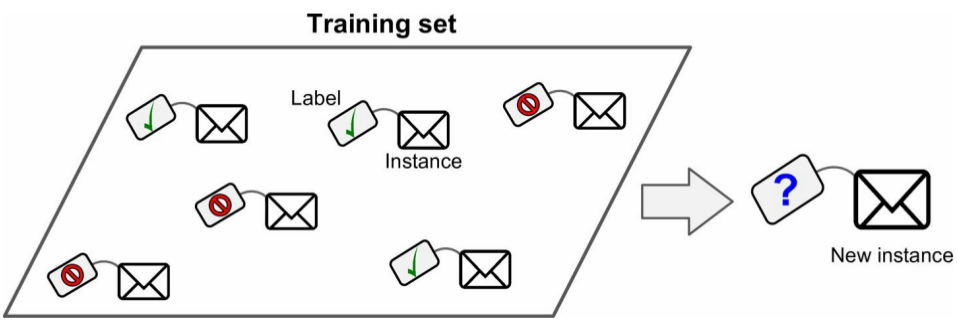
\includegraphics[width=0.30\linewidth]{figuras/supervisedLearning.png}
	\caption{Aprendizaje supervisado}
	\label{AS}
\end{figure}

Una tipica tarea en el aprendizaje supervisado es la clasificacion. El filtrador de spam del correo electronico es un buen ejemeplo de esto: este se entrena con muchos ejemplos de correos electronicos junto con su clase (spam o no spam), y debe aprender a clasificar los nuevos correos electronicos.

\textbf{Algoritmos de Aprendizaje Supervisado}  \\
\begin{itemize}
    \item K-Nearest Neighbors
    
    \item Regresion Lineal
    
    \item Refresion Logica
    
    \item Máquinas de Vectores de Soporte
    
    \item Arboles de decision y bosques aleatorios
    
    \item Redes Neuronales
    
\end{itemize}

\subsection{Aprendizaje no supervisado}
En el aprendizaje no supervisado, los datos de entrenamiento no estan etiquetados. Los sistemas intentan aprender sin un maestro.

\begin{figure}[ht]
	\centering
	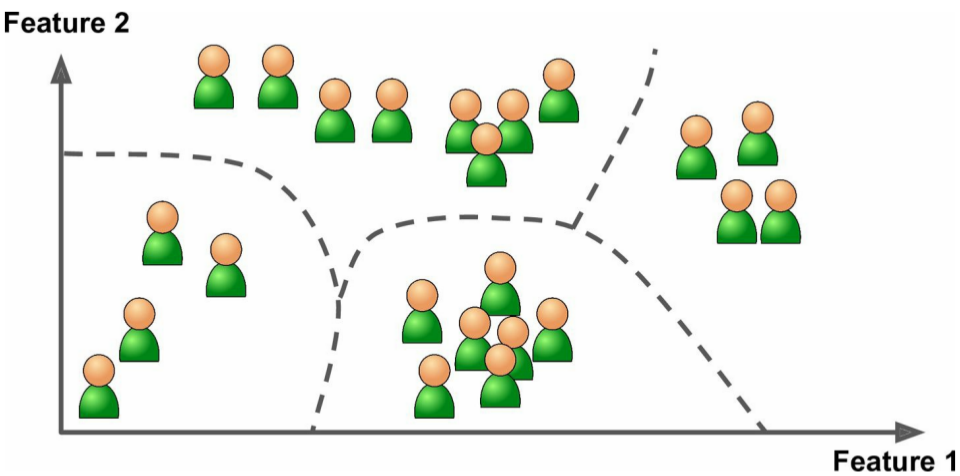
\includegraphics[width=0.30\linewidth]{figuras/clustering.png}
	\caption{Aprendizaje No Supervisado}
	\label{ANS}
\end{figure}

\textbf{Algoritmos de Aprendizaje No Supervisado} 

\begin{itemize}
    \item Agrupamiento
    	\begin{itemize}
    		\item K-Means
   			\item Hirerchical Cluster Analysis (HCA)
    		\item Expectation Maximization
		\end{itemize}
    \item Visualizacion y reduccion de la dimensionalidad
    	\begin{itemize}
    		\item Principal Component Analysis (PCA)
   			\item Kernel PCA
    		\item Locally-Linear Embedding (LLE)
    		\item t-distributed Stochastic Neighbor Embedding (t-SNE)
		\end{itemize}
    \item Aprendizaje de las reglas de asociacion
    	\begin{itemize}
    		\item Apriori
   			\item Eclat
		\end{itemize}
\end{itemize}

\subsection{Aprendizaje Semisupervisado}

Algunos algoritmos pueden tratar con datos de entrenamiento parcialmente etiquetados, normalmente muchos datos sin etiquetar y un poco de datos etiquetados. Esto se llama aprendizaje semisupervisado. Algunos servicios de alojamiento de fotos, como Google Photos, son buenos ejemplos de ello. Una vez que cargues todas tus fotos familiares en el servicio, reconocerá automáticamente que la misma persona A aparece en las fotos 1, 5 y 11, mientras que otra persona B aparece en las fotos 2, 5 y 7. Esta es la parte no supervisada del algoritmo (clustering). Ahora todo lo que el sistema necesita es que le digas quiénes son estas personas. Sólo una etiqueta por persona, 4 y es capaz de nombrar a todos en cada foto, lo que es útil para buscar fotos.

\begin{figure}[ht]
	\centering
	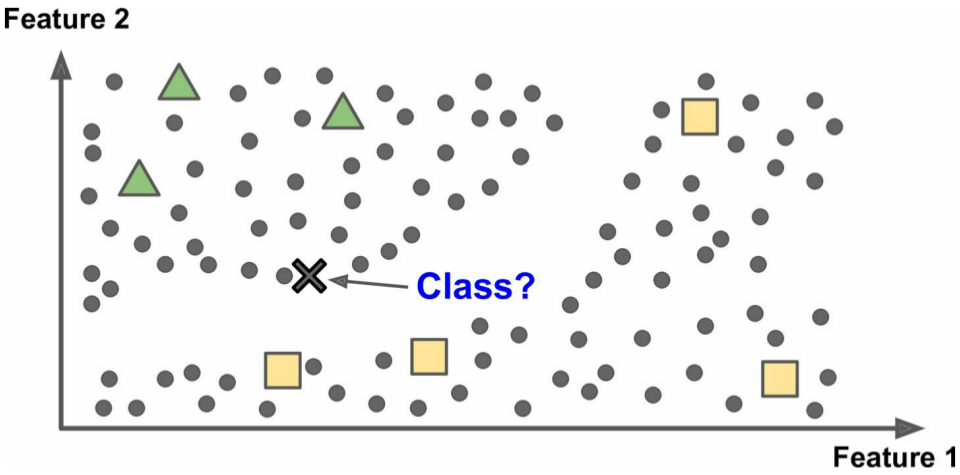
\includegraphics[width=0.30\linewidth]{figuras/semisupervised.png}
	\caption{Aprendizaje Semisupervisado}
	\label{ASS}
\end{figure}

La mayoría de los algoritmos de aprendizaje semisupervisados son combinaciones de algoritmos supervisados y no supervisados. Por ejemplo, las redes de creencias profundas (DBN, por sus siglas en inglés) se basan en componentes no supervisados llamados máquinas Boltzmann restringidas (RBM, por sus siglas en inglés) apiladas unas encima de otras. Los mecanismos para encuadernación con anillos se capacitan secuencialmente de manera no supervisada, y luego se perfecciona todo el sistema utilizando técnicas de aprendizaje supervisado.


\subsection{Aprenizaje Por Refuerzo}
El Aprendizaje de Refuerzo (RL) se refiere a un tipo de método de Aprendizaje Automático en el cual el agente recibe una recompensa retardada en el siguiente paso del tiempo para evaluar su acción previa. Se utilizaba sobre todo en juegos (por ejemplo, Atari, Mario), con un rendimiento igual o incluso superior al de los humanos. Recientemente, a medida que el algoritmo evoluciona con la combinación de redes neuronales, es capaz de resolver tareas más complejas, como el problema del péndulo.

Típicamente, una configuración de RL está compuesta de dos componentes, un agente y un entorno:

\begin{figure}[ht]
	\centering
	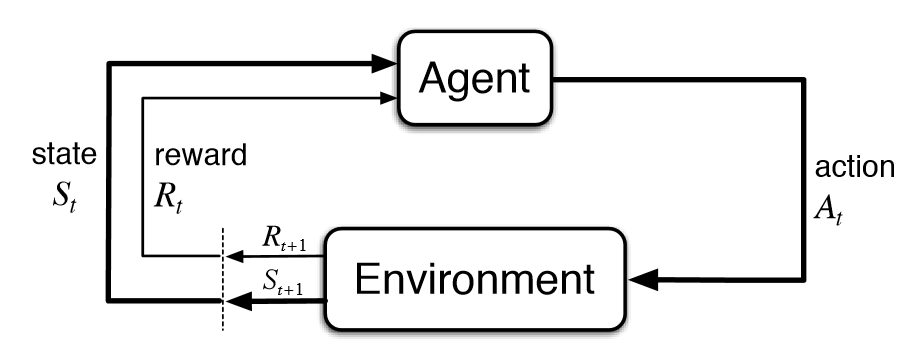
\includegraphics[width=0.30\linewidth]{figuras/reinforcementLearning.png}
	\caption{Configuracion del Aprendizaje por refuerzo}
	\label{ASS}
\end{figure}


Entonces el entorno se refiere al objeto sobre el que el agente está actuando (por ejemplo, el propio juego en el juego de Atari), mientras que el agente representa el algoritmo. El entorno comienza enviando un estado al agente, que luego se basa en su conocimiento para tomar una acción en respuesta a ese estado. Después de eso, el entorno envía un par de estado siguiente y la recompensa de vuelta al agente. El agente actualizará sus conocimientos con el premio devuelto por el medio ambiente para evaluar su última acción. El bucle continúa hasta que el entorno envía un estado terminal, que termina en episodio.

La mayoría de los algoritmos de RL siguen este patrón.

\textbf{Elementos dentro de un algoritmo de aprendizje por refuerzo: }

 \begin{itemize}
  
  \item{ } \textbf{Accion (A): } Todos los movimientos posibles que el agente puede hacer

  \item{ } \textbf{Estado (S): } Situación actual devuelta por el medio ambiente.
	 
  \item{ } \textbf{Recompenza (R): } Un retorno inmediato desde el entorno para evaluar la última acción. 
  		
  \item{ } \textbf{Politica ($\pi$): }  La estrategia que el agente emplea para determinar la siguiente acción basada en el estado actual.
  
  \item{ } \textbf{Valor (V): }  El rendimiento esperado a largo plazo con descuento, a diferencia de la recompensa a corto plazo R. V$\pi$(s) se define como el rendimiento esperado a largo plazo de la actual política de extinción del estado $\pi$.
  
  \item{ } \textbf{valor Q or accion-valor (Q): }   El valor Q es similar al valor V, excepto que toma un parámetro extra, la acción actual a. Q$\pi$(s, a) se refiere al retorno a largo plazo del estado actual s, tomando la acción a bajo la política $\pi$.
  
  \end{itemize}
  
\textbf{Libre de Modelo vs Basado en Modelo: }

El modelo representa la simulación de la dinámica del entorno. Es decir, el modelo aprende la probabilidad de transición T(s1|(s0, a)) del par de estado actual s0 y la acción a al siguiente estado s1. Si la probabilidad de transición se aprende con éxito, el agente sabrá la probabilidad de entrar en un estado específico dado el estado actual y la acción. Sin embargo, los algoritmos basados en modelos se vuelven poco prácticos a medida que crece el espacio de estado y el espacio de acción (S * S * A, para una configuración tabular).

Por otro lado, los algoritmos sin modelos se basan en pruebas y errores para actualizar sus conocimientos. Como resultado, no requiere espacio para almacenar toda la combinación de estados y acciones. Todos los algoritmos discutidos en la siguiente sección caen dentro de esta categoría.

\textbf{Con-Politica vs Sin-Politica }

Un agente con-politica aprende el valor basado en su acción actual a derivada de la política actual, mientras que su contraparte sin-politica lo aprende basado en la acción a* obtenida de otra política. En Q-learning, tal política es la política codiciosa.

\subsection{Algoritmo Q-Learning}

Q-Learning es un algoritmo de Aprendizaje Por Refuerzo libre de politicas y modelos basado en la conocida ecuacion de Bellman:

\begin{figure}[ht]
	\centering
	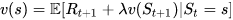
\includegraphics[width=0.30\linewidth]{figuras/bellman.png}
	\label{bellman}
\end{figure}

E en la ecuación anterior se refiere a la expectativa, mientras que $\lambda$ se refiere al factor de descuento. Podemos reescribirlo en forma de valor Q:

\begin{figure}[ht]
	\centering
	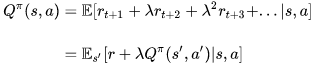
\includegraphics[width=0.30\linewidth]{figuras/qBellman.png}
	\label{qbellman}
\end{figure}

El valor óptimo de Q, indicado como Q*, puede expresarse como:

\begin{figure}[ht]
	\centering
	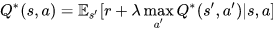
\includegraphics[width=0.30\linewidth]{figuras/qvalue.png}
	\label{qvalue}
\end{figure}

El objetivo es maximizar el valor Q.

\subsection{Redes Neuronales}

Una red neuronal artificial (RNA) es un modelo computacional basado en la estructura y funciones de las redes neuronales biológicas. La información que fluye a través de la red afecta a la estructura de la RNA porque una red neuronal cambia -o aprende, en cierto sentido- basándose en esa entrada y salida.

Las RNA se consideran herramientas de modelado de datos estadísticos no lineales en las que se modelan las complejas relaciones entre entradas y salidas o se encuentran patrones.

La RNA también se conoce como red neuronal.



Una RNA tiene varias ventajas, pero una de las más reconocidas es el hecho de que puede aprender de la observación de conjuntos de datos. De esta forma, la RNA se utiliza como una herramienta de aproximación de función aleatoria. Estos tipos de herramientas ayudan a estimar los métodos más rentables e ideales para llegar a las soluciones mientras se definen las funciones o distribuciones de computación. ANN toma muestras de datos en lugar de conjuntos de datos completos para llegar a soluciones, lo que ahorra tiempo y dinero. Las RNA se consideran modelos matemáticos bastante simples para mejorar las tecnologías de análisis de datos existentes.

Las RNA tienen tres capas interconectadas. La primera capa consiste en neuronas de entrada. Esas neuronas envían datos a la segunda capa, que a su vez envía las neuronas de salida a la tercera capa.

Entrenar una red neural artificial implica elegir entre modelos permitidos para los que existen varios algoritmos asociados.

\begin{figure}[ht]
	\centering
	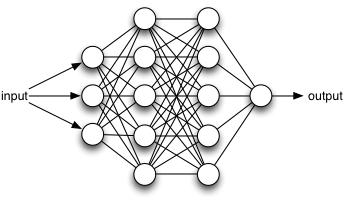
\includegraphics[width=0.30\linewidth]{figuras/neuralNetwork.png}
	\label{qvalue}
\end{figure}

\textbf{Perceptron}

Existen varios modelos para representar una red neuronal. Estos modelos difieren también en los modelos matemáticos. El modelo inicial y más sencillo de entender es el conocido como Pecepron.

Los perceptrones fueron desarrollados en las décadas de 1950 y 1960 por el científico Frank Rosenblatt.  Un perceptrón toma varias entradas binarias, $x1,x2,...,$ y produce una sola salida binaria: 

\begin{figure}[ht]
	\centering
	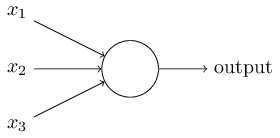
\includegraphics[width=0.30\linewidth]{figuras/perceptron.png}
	\label{qvalue}
\end{figure}

En el ejemplo mostrado el perceptrón tiene tres entradas, $x1,x2,x3.$ En general podría tener más o menos entradas. Rosenblatt propuso una regla simple para calcular el resultado. Introdujo pesos, $w1,w2,...,$ números reales que expresan la importancia de las respectivas entradas a la salida

  La salida de la neurona, 0 o 1, se determina por si la suma ponderada $\sum_{j} w_{j} x_{j} $ es menor o mayor que algún valor umbral. Al igual que los pesos, el umbral es un número real que es un parámetro de la neurona. Para ponerlo en términos algebraicos más precisos: 
  
  \begin{figure}[ht]
	\centering
	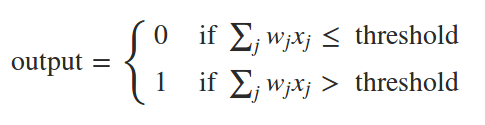
\includegraphics[width=0.30\linewidth]{figuras/perceptron_formula.png}
	\label{qvalue}
\end{figure}
  
 Simplifiquemos la forma en que describimos los preceptrones. La condición $\sum_{j} w_{j} x_{j} > threshold$  es engorroso, y podemos hacer dos cambios notacionales para simplificarlo. El primer cambio es escribir $\sum_{j} w_{j} x_{j} $ como un producto punto, $ w * x \equiv \sum_{j} w_{j} x_{j} $ donde w y x son vectores los cuales componen los pesos y las entradas, respectivamente. El segundo cambio es mover el umbral al otro lado de la desigualdad, y reemplazarlo por lo que se conoce como el sesgo del perceptrón, $ b \equiv -threshold $. Usando el sesgo en lugar del umbral, la regla del perceptrón puede ser reescrita: 
 
   \begin{figure}[ht]
	\centering
	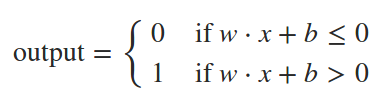
\includegraphics[width=0.30\linewidth]{figuras/perceptron_formula_2.png}
	\label{qvalue}
\end{figure}
 
Se puede pensar en el sesgo como una medida de lo fácil que es conseguir que el perceptrón emita un 1. O para decirlo en términos más biológicos, el sesgo es una medida de lo fácil que es conseguir que el perceptrón se dispare. Para un perceptrón con un sesgo realmente grande, es extremadamente fácil para el perceptrón emitir un 1. Pero si el sesgo es muy negativo, entonces es difícil para el perceptrón emitir un 1
 
 En la red de abajo, la primera columna de percepciones - lo que llamaremos la primera capa de percepciones - es tomar tres decisiones muy simples, sopesando la evidencia de entrada. ¿Qué hay de las percepciones en la segunda capa? Cada una de esas percepciones está tomando una decisión sopesando los resultados de la primera capa de la toma de decisiones. De esta manera un perceptrón en la segunda capa puede tomar una decisión a un nivel más complejo y abstracto que los perceptrones en la primera capa. Y el perceptrón de la tercera capa puede tomar decisiones aún más complejas. De esta manera, una red de múltiples capas de percepciones puede participar en la toma de decisiones sofisticadas.
 
\begin{figure}[ht]
	\centering
	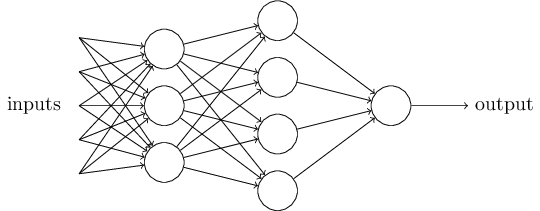
\includegraphics[width=0.30\linewidth]{figuras/net.png}
	\label{qvalue}
\end{figure}


\subsection{TensorFlow}

TensorFlow es una librería de software de código abierto para computación numérica usando gráficas de flujo de datos. Fue desarrollado originalmente por el equipo de Google Brain dentro de la organización de investigación Machine Intelligence de Google para el aprendizaje automático y la investigación de redes neuronales profundas, pero el sistema es lo suficientemente general como para ser aplicable en una amplia variedad de otros dominios también.

TensorFlow es multiplataforma. Funciona en casi todo: GPUs y CPUs -incluyendo plataformas móviles y embebidas- e incluso unidades de procesamiento tensorial (TPUs), que son hardware especializado para realizar cálculos tensores.

\textbf{Modelos de Ejecucion de TensorFlow: Ejecucion de Grafos computacionales }

El aprendizaje automático puede volverse complejo rápidamente, y los modelos de aprendizaje profundo pueden hacerse grandes. Para muchos gráficos de modelos, necesita capacitación distribuida para poder iterar dentro de un marco de tiempo razonable. 
Con Tensorflow puede escribir código para construir un gráfico de cálculo, luego ejecutarlo. El gráfico es una estructura de datos que describe completamente el cálculo que se desea realizar.

Tiene las siguientes ventajas:

  \begin{itemize}
  
  \item{ }Es portátil, ya que el gráfico puede ejecutarse inmediatamente o guardarse para su uso posterior

  \item{ }Puede funcionar en múltiples plataformas: CPUs, GPUs, TPUs, móviles, embebidos. 
  		
  \item{ }Es transformable y optimizable, ya que el gráfico puede ser transformado para producir una versión más óptima para una plataforma determinada. Además, se pueden realizar optimizaciones de memoria o de cálculo y realizar compensaciones entre ellas.  
  		 
   \item{ }Soporte para ejecución distribuida

  \end{itemize}
  
\textbf{TensorBoard}

Tensorboard es un conjunto de aplicaciones web para inspeccionar, visualizar y comprender las ejecuciones y gráficos de TensorFlow. Puede usar TensorBoard para ver las gráficas de su modelo TensorFlow y acercarse a los detalles de las subsecciones de las gráficas.
Puede trazar métricas como la pérdida y la precisión durante una ejecución de entrenamiento; mostrar visualizaciones de histogramas de cómo un tensor está cambiando con el tiempo; mostrar datos adicionales, como imágenes; recopilar metadatos de tiempo de ejecución para una ejecución, como el uso total de memoria y las formas de tensores para los nodos; y más.

\begin{figure}[ht]
	\centering
	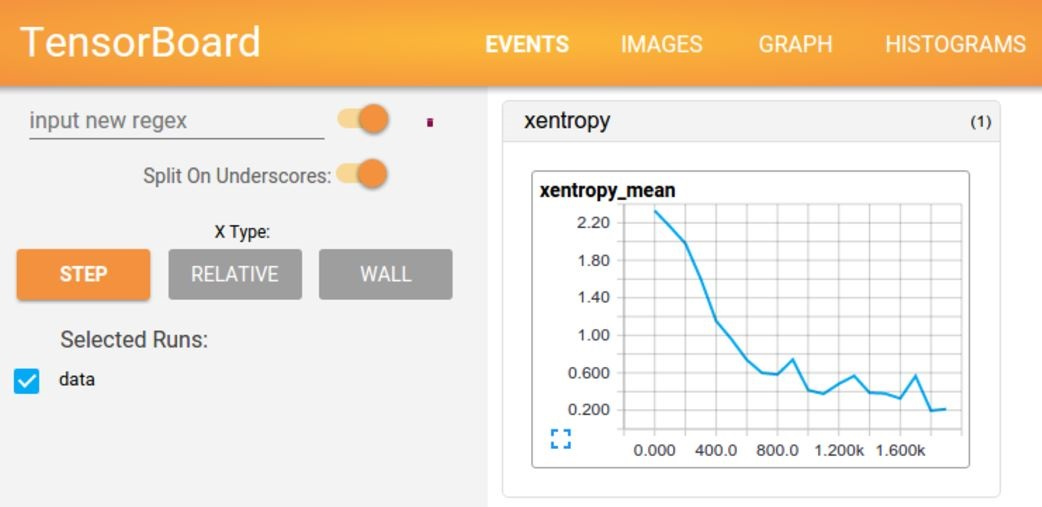
\includegraphics[width=0.30\linewidth]{figuras/tensorboard.jpg}
	\label{qvalue}
\end{figure}


\textbf{Computacion basado en Grafos:}

Tensorflow es un sistema de programación en el que los cálculos computacionales se representan en forma de gráfos. Los nodos en el grafo se llaman ops (abreviatura de operaciones) - Una operación toma cero o más tensores, realiza una cierta operación computacional y produce cero o más tensores. Un tensor es un conjunto multidimensional y estandarizado.


\begin{figure}[ht]
	\centering
	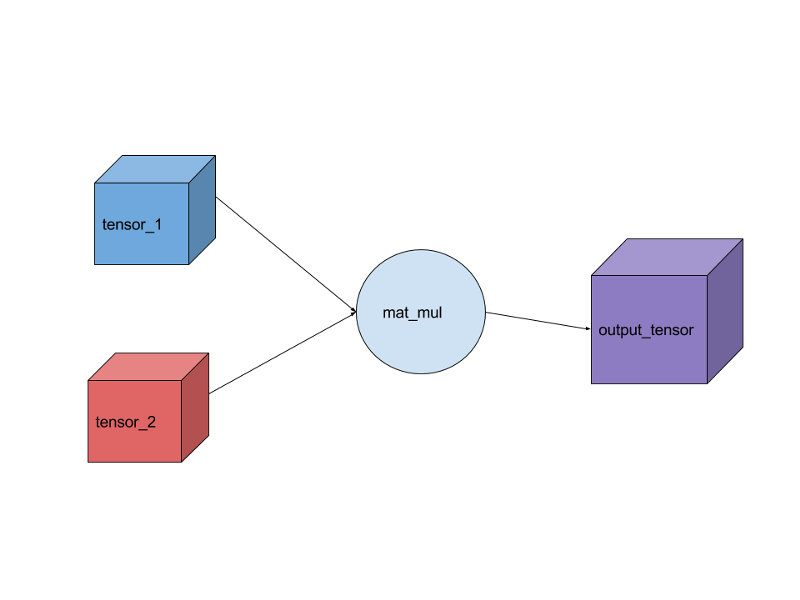
\includegraphics[width=0.30\linewidth]{figuras/tf1.png}
	\label{qvalue}
\end{figure}

Los programas Tensorflow suelen estructurarse en una fase de construcción y una fase de ejecución que utiliza una sesión para ejecutar operaciones en el gráfico.

Por ejemplo, es común crear un gráfico para representar y entrenar una red neuronal en la fase de construcción, y luego ejecutar repetidamente un conjunto de operaciones entrenadas en la fase de ejecución.

Para construir un gráfo, se parte de los ops que no requieren ninguna entrada (source ops), como una constante, y pasa su salida a otro ops para realizar el cálculo computacional.

El constructor de operaciones en la librería Python devuelve los objetos que se mantienen para la salida de las operaciones construidas. Puede pasarlos a otras operaciones construidas para usarlos como entradas.

La librería Python para TensorFlow tiene una gráfica por defecto que añade nodos a los builders ops. El gráfico por defecto es suficiente para muchas aplicaciones.

\subsection{OpenAI gym}

Gym es un juego de herramientas para desarrollar y comparar algoritmos de aprendizaje de refuerzo. No hace suposiciones sobre la estructura de su agente, y es compatible con cualquier biblioteca de cálculo numérico, como TensorFlow o Theano.

La biblioteca gym es una colección de problemas de pruebas - entornos - que puede utilizar para elaborar sus algoritmos de aprendizaje de refuerzo. Estos entornos tienen una interfaz compartida que permite escribir algoritmos generales.
%\clearpage
%\section{Desarrollo del problema}
Para la aplicacion de lo visto en el marco teorico se veran ahora tres aplicaciones del algoritmo de Q-Learning con dos diferentes problemas que son parte de los entornos ofrecidos por la biblioteca OpenAI los cuales se describen a continuacion:

\subsection{Entorno FrozenLake-v0}
FrozenLake-v0 es un entorno estocastico con un espacio de 16 estados y 4 posibles acciones.

El agente controla el movimiento de un personaje en un mundo de cuadrícula. Algunas fichas de la cuadrícula son accesibles para caminar, y otras conducen a que el agente caiga al agua. Además, la dirección de movimiento del agente es incierta y solo depende parcialmente de la dirección elegida. El agente es recompensado por encontrar un camino transitable a una ficha de meta.

El entorno esta descrito con el siguiente enunciado:

El invierno esta aqui. Tú y tus amigos estaban lanzando un frisbee en el parque cuando hiciste un lanzamiento salvaje que dejó el frisbee en el medio del lago. El agua está mayormente congelada, pero hay algunos agujeros donde el hielo se derritió. Si entras en uno de esos agujeros, caerás en el agua helada. En este momento, hay una escasez internacional de frisbee, por lo que es absolutamente imprescindible que navegues por el lago y recuperes el disco. Sin embargo, el hielo es resbaladizo, por lo que no siempre te moverás en la dirección que deseas.

El tablero esta descrito usando una regilla como la siguiente:

\begin{figure}[ht]
	\centering
	\includegraphics*[width=6cm,height=6cm,keepaspectratio]{figuras/Frozen-Lake} 
	\caption{Tablero del FrozenLake}
	\label{fig:Frozen-Lake}
\end{figure}

S: Punto inicial, seguro.
F: Superficie congelada, seguro.
H: Hoyo, cai en las profunidades.
G: Meta, donde el frisbee esta localizado.

\subsection{Q-Table: Solucion a FrozenLake-v0 con la ayuda de tablas de decision}

El algoritmo Q-Learning es un algoritmo perteneciente a la familia de los algoritmos de aprendizaje por refuerzo, es uno de los mas usados en esta rama siendo fuera de politica y de metodo, por ello su flexibilidad al momento de elegir un metodo para elegir la mejor accion a tomar por el agente. El algoritmo tiene algunas variantes dependiendo en su aplicacion siendo dos de estas 1) por medio de tablas de decision que son llenadas y refinidas  conforme para el tiempo de ejecucion y 2) aplciando complejos modelso como los son las redes neuronales, en esos problemas en los cuales almacenar valores en las tablas no es una accion factible ni escalable.

Una tabla Q esta dada por los estados: los posibles estados que puede tomar el entorno y por el numero de acciones que puede realizar.

Siendo asi en el problema de FrozenLake-v0 teniendo una tabla Q de 16x4 en la cual se guardan valores que deciden que accion tomara el agente para llegar hasta su objetivo.

La formula que se aplica en este tipo de problemas para llenar o actualizar la tabla en cada uno de los episodios es la siguiente:

\begin{figure}[ht]
	\centering
	\includegraphics*[width=8cm,height=4cm,keepaspectratio]{figuras/formula} 
	\label{fig:formula Q-Tables}
\end{figure}

\textbf{Desarrollo algoritmico del problema: }

Para la resolucion de este se utilizo el legnuaje de programacion Python 3.6 junto con las biblitecas de Numpy y OpenAI gym, ademas de Matplotlit para graficar los resultados.


\begin{figure}[ht]
	\centering
	\includegraphics*[width=15cm,height=20cm,keepaspectratio]{figuras/q_table_1} 
	\label{fig:formula Q-Tables}
\end{figure}

\begin{figure}[ht]
	\centering
	\includegraphics*[width=15cm,height=20cm,keepaspectratio]{figuras/q_table_2} 
	\label{fig:formula Q-Tables}
\end{figure}

\begin{itemize}
    \item Lineas 1-6: Se encargar de importar los paquetes necesarios de las bilbiotecas
    \item Linea 8: Prepara el entorno FrozenLake el cual establece una matriz de 4 x4
    \item Linea 10: declara el array Q el cual es inicializado con ceros y el tamaño de la matriz mencionada anteriormente
    \item Linea 12-14: Configura las constantes que son el factor de aprenizaje (lr) y el factor de descuento (y), asi como el numero total de episodios que son obtenido por el entrenamiento
    \item Las listas declaradas en las lineas 16 y 17 se usan para almacenar el total de pasos que son realizados en cada episodio y el total de recompenzas en cada episodio
    \item Lineas 19-42: Denota el ciclo atraves el cual son puestos en marcha los episodios
    \item Lineas 20-23: El estado del entorno es reseteado a su posicion original, la variable rAll en una variable acumuladora la cual agrega todas las recompenzas ganadas en cada episodio, la variable d es una variable booleana la cual indica si el agente cayo o llego a su destino y la variable j es una variable contadora la cual cuenta el numero de pasos en cada episodio
    \item Lineas 26-38: Indica el espacio en el tiempo en donde el agente da 100 pasos para moverse alrededor hasta que llegue al destino o caiga dentro de un hoyo
    \item Linea 29: aplica un ruido al valor de accion
    \item Linea 30: Llama a la funcion step(), la cual retorna cuatro valores los cuales son: el siguiente estado, la recompenza dada por esa accion, un valor booleano el cual indica si el agente cao dentro de un hoyo o llego al objetivo, y un valor que indica informacion extra para debugging
    \item Linea 31: se usa la formula de Q-Learning usando las variables previamente afectadas por la siguiente accion tomada
    \item Linea 32: acumula la recompenza ganada
    \item Linea 33: El viejo estado es rempelzado con el nuevo
    \item Linea 35: Muestra el entorno y el movimiento del agente graficamente
    \item Linea 37: Compara si la variable indicando que el episodio terminado es verdadera
    \item Linea 40 y 41: Agrega informacion colectada de los pasos y las recompenzas al final de cada episodio
    \item Lineas 43-45: imprime los resultados finales
\end{itemize}

\subsection{Q-Network: Solucion al entorno FrozenLake-v0 aplicando redes neuronales artificiales}

La tabla Q para almacenar valores que influyen en la toma de desciones por parte del agente es una buena aplicacion, pero la desventaja que existe es que en problemas/entornos mas complejos y algunos de la vida real el numero de posibles acciones aumenta drasticamente y en ello una tabla de valores no es una manera viable y ademas poco escalable para resolver ese tipo de problemas. Por ello en temas complejos existen metodos compeljos como lo son las redes neuronales que son las que predicen una buena accion basado en experiencia anterior y consumen menos recursos de memoria lo cual con las tablas queda corto.

Para este problema se tiene el mismo problema, entorno. pero en esta ocasion se utiliza una red neuronal gracias a la biblioteca TensorFlow. Tensorflow provee y adiciona al entorno mucha mas capacidad gracias a su computacion en grafo.

El objetivo de la red es aprende a como mapear los valores Q sin la necesidad de guardar estos en una tabla.

El grafico de la red neuronal a utilizar se puede replesentar en la siguiente figura:

\begin{figure}[ht]
	\centering
	\includegraphics*[width=10cm,height=10cm,keepaspectratio]{figuras/red} 
	\label{fig:formula Q-Tables}
\end{figure}

\textbf{Desarrollo algoritmico del problema: }

Se utiliza una red neuronal de 16 nodos en la capa de entrada y 4 nodos en la capa de salida.

Un vector con codificacion one-hot toma los estados en la capa de entrada, este vector tiene una medidad de 1x16

Un vector de salida de 1x4 se designa para las salidas de la red y los cuales cada nodo corresponde a una accion posible a tomar por el agente.

Los pesos de la red funcionan como las celdas de la tabla Q teniendo una matriz de 16x4 como resultado de la asignacion de cada nodo de entrada y nodo de salida.

Ademas el metodo de actualizacion es diferente comparado con el Q-Table que se usa una formula para actualizar el valor, en lugar de actualizar directamente la tabla, con la red neuronal se usa backpropagation y una funcion de perdida (la funcion de perdida es la suma de los cuadrados perdidos)

La funcion de perdida sera la suma de los cuadrados de la perdida, donde la diferencia entre el valor Q actual predicho y el valor objetivo es computado y la gradiente pasa a traves de la red.

En el aprendizaje de backpropagation cada vez que se presenta un vector de entrada de una muestra de entrnamiento, el vector de salida se compara con el valor deseado.

El resultado dado de esta comparacion nos dice cuan lejos estamos del valor deseado para una entrada en particular. El objetivo de la backpropagation es minimizar la suma de el error para todas las muestras de entrenamiento, de modo que la red se comporte de una manera mas deseable ajustando los pesos de la red.

\begin{figure}[ht]
	\centering
	\includegraphics*[width=15cm,height=20cm,keepaspectratio]{figuras/q_net1} 
	\label{fig:q_network code 1}
\end{figure}

\begin{figure}[ht]
	\centering
	\includegraphics*[width=15cm,height=20cm,keepaspectratio]{figuras/q_net2} 
	\label{fig:q_network code 2}
\end{figure}

\begin{itemize}
    \item Lineas 1-6: Se importan las bibliotecas gym, numpy, random, tensorflow y matplotlib
    \item Linea 8: Se carga el entorno FrozenLake-v0 desde el metodo make de la biblioteca de gym
    \item Linea 10: Limpia la pila del grafo por defecto y la reinicia
    \item Lineas 12-15: Se establece el modelo de la red neuronal, con 16 nodos en la capa de entrada y 4 nodos en la capa de salida
    	\begin{itemize}
    		\item Linea 12: declara un placeholder en donde se van a introducir los datos de la entrada con una forma del total de nodos en la entrada de la red que en este caso son 16, uno para cada posible estado que pueda tomar el agente
    		\item Linea 13: se declara una variable el cual es un tensor de tamaño 16 x 4 que representan los pesos en la red neuronal, en este caso se les esta asignando un valor aleatorio que va de 0 - 0.0099999
    		\item Linea 14: Se declara un Op con una operacion de multiplicacion de matrices las cuales corresponen a las entradas por los pesos
    		\item Linea 15: Se declara un Op para elegir la salida con mayor valor, es decir la elegida por el agente como la mejor accion tomada
    	\end{itemize}
    \item Linea 17-20: Es bloque se utiliza para optimizar la red neuronal y ajustarla para de esta forma realiza aprendizaje.
    \item Lineas 24-26: Se establecen los parametros de aprendizaje, asi como el numero de episodios con los que contara la red para aprender y obtener en el mejor camino para llegar al objetivo
    \item Linea 27: Se establece una ruta para guardar el modelo de tensorflow para poserior visualizacion en tensorboard
    \item Lineas 29-30: Se crean dos listas las cuales guardan el acumulado del total de recompenzas y el total de pasos realizados en cada episodio
    \item Lineas 31-67: Se establece una sesion de tensorflow para ejecutar el modelo previamente creado
    \item Linea 33: Se ejecuta el Op en el cual se inicializan todas las variables previamente declaradas
    \item Linea 34: Con esa instruccion Tensorflow guarda de manera local en un archivo el modelo del grafo realizado en el programa para abrirlo posteriormente en la herramienta tensorboard, ademas se especifica la ruta antes establecida en la variable logs\_path
	\item Lineas 36-67: bucle de los episodios realizados que en este caso son 2000
	\item Linea 37: Esta instruccion hace que el agente en el entorno actual regrese al estado inicial del mismo
	\item Linea 38-40: reinicia las variables contadora de los pasos realizados por episodio y el total de recompenzas dadas por dicho episodio, ademas que pone en falso la variable que determina si el episodio termino
	\item Lineas 42-64: Determina el bucle en el cual se realizan determinados pasos para cada episodio, que en este caso son 100
	\item Linea 45: Ejecuta los Ops los cuales se encargan de la multiplicacion de las matrices de los pesos por las entradas, asi como codifica de forma one-hot las entradas, asi como toma la mejor accion a tomar en dicho procedimiento definido por la red
	\item Linea 62-64: Esas acciones definen si el agente toma una accion random, dandonde de inicio 10 \% de probabilidad de tomar una de estas, y esto va reduciendose conforme pasen episodios
	\item Linea 50: se toma determina accion definida por la red en la linea 45 y esta sele pasa al entorno, retornando este los siguientes valores: siguiente estado del agente, recompenza dada, variable que determina si el entorno fue terminado e informacion de debbugin
	\item Linea 52: Obtiene los valores de salida para la siguiente accion
	\item Lineas 54-56: Optiene el valor optimo para la accion realizada basandose en el actual valor Q (que son las salidas de la red) y el siguiente
	\item Linea 58: Optimiza la red, en este proceso se podria decir que la red esta aprendiendo, este Op ejecuta el bloque de codigo anterior definido en la fase de construccion, tomando una formula sacando el valor de error y optimizando los pesos de la red gracias a la gradiente descendente
	\item Linea 59: Se almacena/acumula la recompenza ganada en el presente episodio 
	\item Linea 60: El estado actual, toma el siguiente optenido por el entorno gracias a la bilbioteca OpenAI gym
	\item Lineas 62-64: Condicional que termina el ciclo del episodio si el entorno devuelve true en la variable que almacena si el entorno termino
	\item Linea 63: modifica el valor de la probabilidad de tomar una accion aleatoria en las lineas 100-101 reduciendolo
	\item Linea 66-67: Agrega a las listas que almacenan los datos de pasos totales y recompenzas dadas en el problemas las variables que almacenan dicha informacion en cada episodio
	\item Lineas 69-72: Imprime el rednimiento dado por la aplicacion y la red con una grafica con la ayuda de la bilbioteca de matplotlib
\end{itemize}

\subsection{Entorno NChain-v0}

NChain-v0 es otro entorno de la bilbioteca de OpenAI gym el cual cuenta con un espacio de 5 estados y 2 posibles acciones.

\textbf{Descripcion:}

\begin{itemize}
    \item Se tiene una cadena de 5 estados
    
    \item Los arcos son rotulados con las acciones que causa la transicion de estado y su recompenza asociada
    
    \item Visualmente la accion abstracta 1 hace que la accion a en el entorno se lleve a cabo
    
    \item La accion abstracta 2 causa la accion en el entorno b
    
    \item Con posibilidad de 0.2, el agente "se desliza" y su accion tiene el efecto opuesto
    
    \item El comportamiento optimo es elegir siempre la accion 1 (aunque esto a veces da como resultado las transiciones etiquetadas con b)
    
    \item Una vez que se alcanza el estado 5, se recibe una recompenza de 10 antes que el agente resbale y regrese al estado 1
    
    \item cada que cae la accion 2 el agente vuelve al estado 1 del entorno
    
\end{itemize}

Este problema requiere de una exploracion efectiva y una estimacion precisa de la recompenza descontada

\textbf{Acciones:}

\begin{itemize}
    \item a o 1.- Hacia adelate
    
    \item b o 2.- Hacia atras
    
\end{itemize}

\textbf{No. Estados:}

\begin{itemize}
    \item 5
\end{itemize}

\textbf{Recompenzas:}

\begin{itemize}
    \item +0 accion hacia adelante
    \item +2 si se resbala y empeza en el estado 1
    \item +10 si llega al estado 5
\end{itemize}

Graficamente el entorno se veria asi:

\begin{figure}[ht]
	\centering
	\includegraphics*[width=12cm,height=8cm,keepaspectratio]{figuras/nchain} 
	\caption{Tablero del NChain}
	\label{fig:N-Chain}
\end{figure}


\subsection{Solucion al entorno NChain-v0 aplicando redes neuronales}
Para este problema se tiene contemplado reutilizar el problema anteriormente trato en el cual se aplicaba una red neuronal de una capa, en la cual tenia 16 nodos de entrada y 4 nodos de salida.

Para este problema se tienen 2 posibles acciones a tomar las cuales son si el agente va hacia adelante o hacia atras, por los cual se requiere una capa de salida con dos nodos en la red neuronal. Ademas de esto se cuenta con 5 posibles estados que puede tomar el agente, por ello, se tiene una capa de entrada de 5 nodos los cuales representaran estos.

Por lo cual se tienen una capa de entrada con 5 nodos y una capa de salida con 2 nodos, esto da como resultado una matriz de pesos con una forma de 5x2, como lo muestra el siguiente grafico:

\begin{figure}[ht]
	\centering
	\includegraphics*[width=10cm,height=10cm,keepaspectratio]{figuras/red2} 
	\label{fig:red2}
\end{figure}

Este entorno en particular al momento de realizar una accion, no devuelve una variable de terminacion del episodio por ello, no es necesario colocar la condicion que realizaba este proceso como en el codigo del problema anterior. La solucion es muy parecida al problema anterior solo ajustando pequeños detalles para este problema.

\textbf{Desarrollo algoritmico del problema:}


\begin{figure}[ht]
	\centering
	\includegraphics*[width=15cm,height=20cm,keepaspectratio]{figuras/nchain1} 
	\label{fig:nchain code 1}
\end{figure}

\begin{figure}[ht]
	\centering
	\includegraphics*[width=15cm,height=20cm,keepaspectratio]{figuras/nchain2} 
	\label{fig:nchain code 2}
\end{figure}

\begin{figure}[ht]
	\centering
	\includegraphics*[width=15cm,height=20cm,keepaspectratio]{figuras/nchain3} 
	\label{fig:nchain code 3}
\end{figure}

\begin{itemize}
    \item Lineas 1-6: Se importan las bibliotecas gym, numpy, random, tensorflow y matplotlib
    \item Linea 8: Se carga el entorno NChain-v0 desde el metodo make() de la biblioteca de gym
    \item Linea 10: Se reinicia el entorno con el metodo reset() el cual coloca al agente en su posicion origial de inicio 
    \item Linea 12: Limpia la pila del grafo por defecto y la reinicia    
    \item Lineas 14-17: Se establece el modelo de la red neuronal, con 5 nodos en la capa de entrada la cual es llamda 'x' y 2 nodos en la capa de salida como se puede apreciar en la linea 19
    	\begin{itemize}
    		\item Linea 14: declara un placeholder en donde se van a introducir los datos de la entrada con una forma del total de nodos en la entrada de la red que en este caso son 5, uno para cada posible estado que pueda tomar el agente
    		\item Linea 15: se declara una variable el cual es un tensor de tamaño 5 x 2 que representan los pesos en la red neuronal, en este caso se les esta asignando un valor aleatorio que va de 0 - 0.0099999
    		\item Linea 16: Se declara un Op con una operacion de multiplicacion de matrices las cuales corresponen a las entradas por los pesos
    		\item Linea 17: Se declara un Op para elegir la salida con mayor valor, es decir la elegida por el agente como la mejor accion tomada
    	\end{itemize}
    \item Linea 19-22: Es bloque se utiliza para optimizar la red neuronal y ajustarla para de esta forma realiza aprendizaje.
    \item Lineas 26-28: Se establecen los parametros de aprendizaje, asi como el numero de episodios con los que contara la red para aprender y obtener en el mejor camino para llegar al objetivo
    \item Linea 24: Se establece una ruta para guardar el modelo de tensorflow para poserior visualizacion en tensorboard
    \item Lineas 30-31: Se crean dos listas las cuales guardan el acumulado del total de recompenzas y el total de pasos realizados en cada episodio
    \item Lineas 32-65: Se establece una sesion de tensorflow para ejecutar el modelo previamente creado
    \item Linea 34: Se ejecuta el Op en el cual se inicializan todas las variables previamente declaradas
    \item Linea 36: Con esa instruccion Tensorflow guarda de manera local en un archivo el modelo del grafo realizado en el programa para abrirlo posteriormente en la herramienta tensorboard, ademas se especifica la ruta antes establecida en la variable logs\_path
	\item Lineas 38-65: bucle de los episodios realizados que en este caso son 10
	\item Linea 40: Esta instruccion hace que el agente en el entorno actual regrese al estado inicial del mismo
	\item Linea 40-42: reinicia las variables contadora de los pasos realizados por episodio y el total de recompenzas dadas por dicho episodio, ademas que pone en falso la variable que determina si el episodio termino
	\item Lineas 45-65: Determina el bucle en el cual se realizan determinados pasos para cada episodio, que en este caso son 10
	\item Linea 48: Ejecuta los Ops los cuales se encargan de la multiplicacion de las matrices de los pesos por las entradas, asi como codifica de forma one-hot las entradas, asi como toma la mejor accion a tomar en dicho procedimiento definido por la red
	\item Linea 50-51: Esas acciones definen si el agente toma una accion random, teninedo como probabilidad de 10\% a que tome una decision aleatoria, la cual no disminuye conforme pasan los episodios, debido a la facilidad del entorno
	\item Linea 53: se toma determina accion definida por la red en la linea 48 y esta sele pasa al entorno, retornando este los siguientes valores: siguiente estado del agente, recompenza dada, variable que determina si el entorno fue terminado e informacion de debbugin
	\item Linea 55: Obtiene los valores de salida para la siguiente accion
	\item Lineas 57-59: Optiene el valor optimo para la accion realizada basandose en el actual valor Q (que son las salidas de la red) y el siguiente
	\item Linea 61: Optimiza la red, en este proceso se podria decir que la red esta aprendiendo, este Op ejecuta el bloque de codigo anterior definido en la fase de construccion, tomando una formula sacando el valor de error y optimizando los pesos de la red gracias a la gradiente descendente
	\item Linea 62-63: Se almacena/acumula la recompenza ganada en el presente episodio 
	\item Linea 63: El estado actual, toma el siguiente optenido por el entorno gracias a la bilbioteca OpenAI gym
	\item Linea 64-65: Agrega a las listas que almacenan los datos de pasos totales y recompenzas dadas en el problemas las variables que almacenan dicha informacion en cada episodio
	\item Lineas 67-73: Imprime el rendimiento dado por la aplicacion y la red con una grafica con la ayuda de la bilbioteca de matplotlib
\end{itemize}



%\clearpage
%\section{Resultados}

\subsection{Resultados de Q-Table}

La tabla Q al final de 200 episodios quedo de la siguiente manera: 


\begin{figure}[ht]
	\centering
	\includegraphics*[width=10cm,height=10cm,keepaspectratio]{figuras/table_final} 
	\label{fig:valor final Tabla Q}
\end{figure}

El rendimiento el algoritmo esta representado por el siguiente grafico:

\begin{figure}[ht]
	\centering
	\includegraphics*[width=10cm,height=10cm,keepaspectratio]{figuras/plot} 
	\label{fig:plot final}
\end{figure}
%\clearpage
%\section{Conclusiones}

El creciente desarrollo de la computacion ha tenido gran auge debido al poder computacional con el que hoy en dia cuentan nuestros dispositivos. Pero aun asi es corto en comparacion con los problemas aun que nos queda por resolver, problemas que en ocasiones no tienen una solucion en un espacio temporal adecuado.

Afortunadamente los programadores y cientificos de datos estan ideando nuevos metodos para hacerles frente a estos problemas, o para encontrar una solucion B que se acerque al optimo requerido, algunas de estas tecnicas son las de aprendizaje automatico, en las cuales se programan a las computadoras para que estas puedan aprender en base a su experiencia emulando los procesos en los seres vivos.

Como se vio en el presente documento se aplico una solucion relativamente sencilla a un problema en un entorno controlado gracias a la biblioteca gym que pertenece a la organizacion de OpenAI, en el cual se aplicaron algoritmos de aprendizaje por refuerzo y mas puntualmente el algoritmo de Q-Learning. Ademas de esto se aplicaron metodos complejos como lo son las redes neuronales para optimizar la solucion y poder resolverlo en un espacio temporal y espacial mucho mas corto y ademas escalable si el problema crece comparados con los metodos tradicionales de Q-Learning.

Definitivament el aprednizaje automatico y la inteligencia artificial junto con metodos complejos hacen la diferencia ante distintos problemas computacionales a los cuales hoy en dia muchos programadores y cientificos se enfrentan.
%\clearpage
%\addcontentsline{toc}{section}{Índice de figuras}
%\renewcommand\listfigurename{Índice de figuras}

%\listoffigures
%\clearpage
%\addcontentsline{toc}{section}{Índice de cuadros}
%\renewcommand\listtablename{Índice de cuadros}
%\listoftables
%-----------------------------------------------------------------------------------------------------------------
% REFERENCIAS
\clearpage
%\Urlmuskip=0mu plus 1mu\relax
%\addcontentsline{toc}{section}{Referencias} 
%\printbibliography

\end{document}
\grid